\documentclass[12pt,a4paper]{article}
\usepackage[UTF8]{ctex}
\usepackage{geometry}
\usepackage{graphicx}
\usepackage{float}
\usepackage{caption}
\usepackage{subcaption}
\usepackage{enumitem}
\usepackage{hyperref}
\usepackage{fancyhdr}
\usepackage{listings}
\usepackage{xcolor}
\usepackage{amsmath}
\usepackage{amssymb}

\usepackage{booktabs}   
\usepackage{array}     

% 页面设置
\geometry{left=2.5cm,right=2.5cm,top=2.5cm,bottom=2.5cm}

% 图片路径（如果图片放在 media 文件夹下）
%\graphicspath{{media/}}

% 超链接设置
\hypersetup{
	colorlinks=true,
	linkcolor=blue,
	urlcolor=blue,
}

% 页眉页脚
\pagestyle{fancy}
\fancyhf{}
\fancyhead[L]{实验二：软件设计与建模报告}
\fancyhead[R]{杨蕊羽\quad 241220108}
\fancyfoot[C]{\thepage}

% 代码块设置
\lstset{
	basicstyle=\ttfamily\small,
	breaklines=true,
	frame=single,
	numbers=left,
	numberstyle=\tiny,
	tabsize=4,
}

\begin{document}
	
	% ===================== 标题 =====================
	\begin{center}
		{\LARGE \textbf{实验二：软件设计与建模报告}} \\[0.5cm]
		{\large 241220108\quad 杨蕊羽} \\[0.5cm]
		\rule{\textwidth}{0.4pt}
	\end{center}
	
	\section{软件的主要功能}
	
	\subsection{软件概述}
	
	本项目设计并实现一个面向校园二手物品交易场景的校园二手交易系统，
	系统采用角色权限管理机制，将用户划分为买家、卖家和管理员三种角色。不同角色具有不同的业务操作权限，通过商品管理、商品查询、商品审核、预约与交易管理与日志管理等功能模块，实现校园二手交易业务的完整流程。
	
	\subsection{用户与权限管理}
	
	用户与权限管理模块负责系统用户的注册、登录和角色权限控制。主要功能包括：
	\begin{itemize}
		\item \textbf{用户注册：}用户填写用户名、密码和联系电话，选择对应的用户角色，完成账号注册。
		\item \textbf{用户登录：}卖家、买家用户通过用户名和密码进行登录。	\item \textbf{管理员邀请码验证：}管理员注册时必须提供一次性邀请码，邀请码成功使用后不能再次使用。
		\item \textbf{角色管理：}系统支持买家、卖家和管理员三种角色，根据用户角色限制其可执行的操作。
		\item \textbf{权限验证：}在执行商品管理、预约交易和管理员操作等业务前，系统检查当前用户是否具有相应权限。
	\end{itemize}
	
	\subsection{商品管理}
	
	商品管理模块主要面向卖家，负责商品信息的创建、修改、审核提交及状态维护。商品具有草稿、待审核、审核驳回、已发布、已预约、卖家已确认、已售出、已下架和违规下架九种状态。
	系统通过商品状态控制相应操作，避免不符合业务规则的状态转换。
	主要功能包括：
	\begin{itemize}
		\item \textbf{创建商品草稿：}卖家按照格式规定填写商品标题、描述、分类、价格、图片和交易地点，保存为草稿。
		\item \textbf{编辑商品信息：}卖家根据商品当前状态，在允许的情况下修改商品信息。
		\item \textbf{提交商品审核：}卖家提交完整的商品信息，系统将商品状态设置为待审核，并生成对应的审核记录。
		\item \textbf{商品下架：}卖家可以对符合条件的已发布商品执行普通下架操作。
		\item \textbf{商品状态管理：}系统根据审核结果、预约交易和管理员违规下架结果维护商品状态。
	\end{itemize}
	
	\subsection{商品查询}
	
	商品查询模块主要面向买家，同时为卖家和管理员提供相应的商品查询能力。主要功能包括：
	\begin{itemize}
		\item \textbf{商品浏览：}买家浏览系统中已发布的商品。
		\item \textbf{商品搜索：}根据商品关键词查询符合条件的商品。
		\item \textbf{条件筛选：}支持按照商品价格区间等条件进行筛选。
		\item \textbf{商品详情查询：}查看商品标题、描述、价格、图片和交易地点等信息。
		\item \textbf{我的商品查询：}卖家查询自己发布的商品。
		\item \textbf{全部商品查询：}管理员根据管理需要查询系统中的商品信息。
	\end{itemize}
	
	\subsection{商品审核}
	
	商品审核与违规处理模块主要面向管理员，负责审核卖家提交的商品以及处理违规商品。主要功能包括：
	\begin{itemize}
		\item \textbf{查询待审核商品：}管理员查询当前等待审核的商品。
		\item \textbf{审核商品：}管理员查看商品提交的信息，决定审核通过或驳回，并在驳回时填写原因。
		\item \textbf{保存审核记录：}每次提交审核都会生成独立的审核记录，保存商品提交内容快照及审核结果。
		\item \textbf{违规下架：}管理员选择违规商品，填写违规原因并执行下架操作。
		\item \textbf{关联记录处理：}违规下架时，系统同步关闭商品当前有效预约以及当前待审核记录（如存在），并保留相关历史记录。
	\end{itemize}
	
	\subsection{预约与交易管理}
	
	预约与交易管理模块负责买家发起预约、卖家处理预约以及交易完成确认，是系统的核心业务模块。主要功能包括：
	\begin{itemize}
		\item \textbf{创建购买预约：}买家选择已发布商品并发起预约。
		\item \textbf{查看预约记录：}买家查看自己发起的预约，卖家查看收到的预约。
		\item \textbf{确认预约：}卖家确认买家的预约请求。
		\item \textbf{拒绝预约：}卖家拒绝不符合交易意向的预约。
		\item \textbf{取消预约：}买家根据预约当前状态取消预约。
		\item \textbf{确认交易完成：}交易双方完成线下交易后，由买家确认交易完成。
		\item \textbf{联系方式查看：}预约经卖家确认后，交易双方可以查看对方的联系方式。
		\item \textbf{违规预约关闭：}商品被管理员违规下架时，系统同步关闭相关有效预约。
	\end{itemize}
	
	\subsection{统计与日志管理}
	
	统计与日志管理模块主要面向管理员，负责记录系统关键业务操作和查询平台运行情况。主要功能包括：
	\begin{itemize}
		\item \textbf{操作日志记录：}记录操作人、操作类型、操作对象、对象编号、操作前后状态、执行结果、操作原因和操作时间。
		\item \textbf{操作日志查询：}管理员查询系统历史操作记录。
		\item \textbf{商品状态统计：}统计不同商品状态下的商品数量。
	\end{itemize}
	
	\section{软件架构 UML 图设计}
	
	\subsection{组件图}

	\begin{figure}[H]
		\centering
		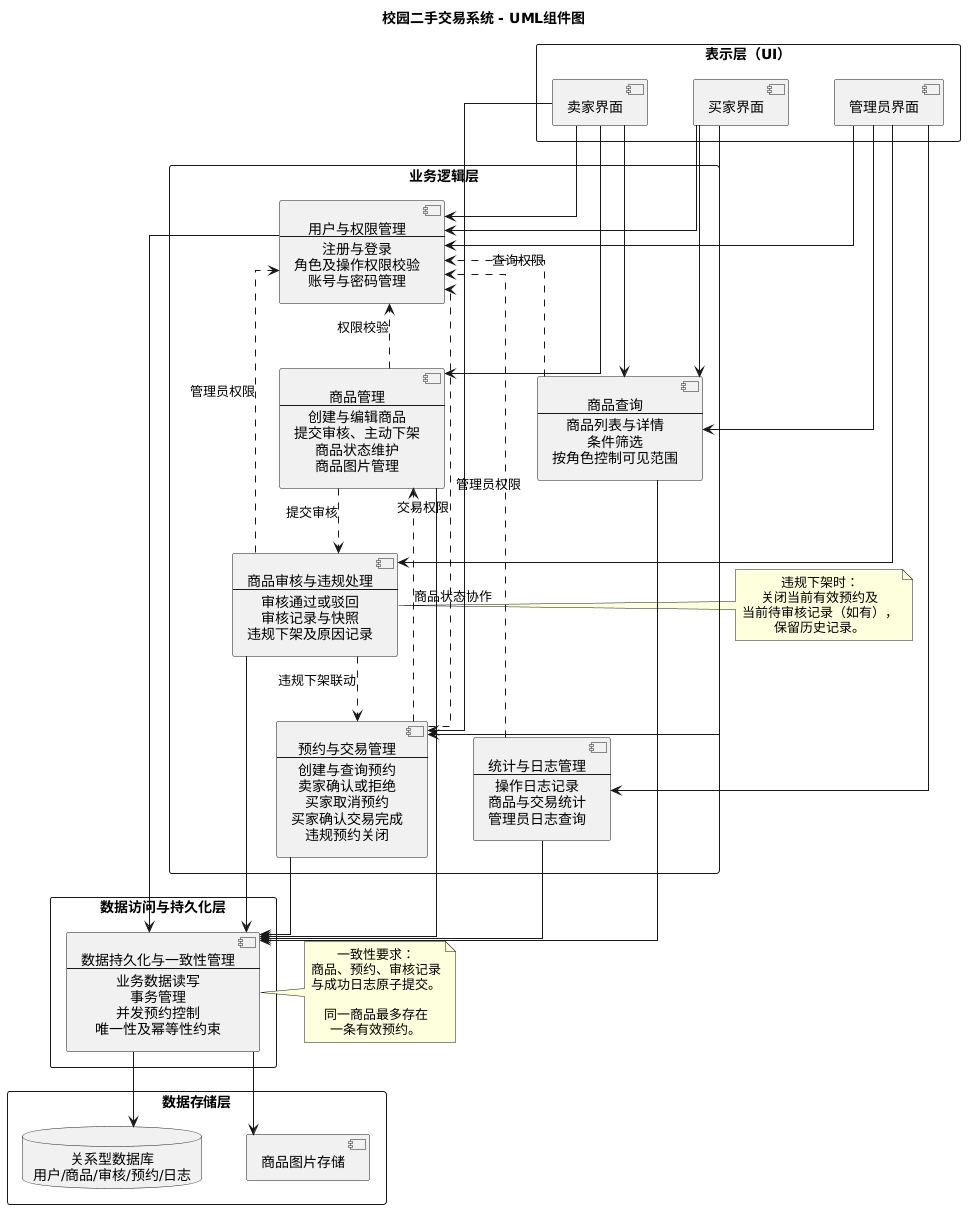
\includegraphics[width=0.92\textwidth]{UML/UML组件图.png}
		\caption{校园二手交易系统 UML 组件图}
		\label{fig:component}
	\end{figure}
	
	本系统采用分层架构设计，将系统划分为表示层（UI）、业务逻辑层、数据访问与持久化层以及数据存储层。系统总体架构如图~\ref{fig:component}所示。
	
	
	\subsubsection{各层的主要职责}
	
	\textbf{表示层：}
	
	表示层负责与用户进行交互，接收用户输入并展示系统处理结果。根据系统的三种用户角色，表示层划分为：
	\begin{itemize}
		\item \textbf{买家界面：}提供商品浏览、商品筛选、商品详情查询、购买预约和交易完成确认等功能。
		\item \textbf{卖家界面：}提供商品发布、商品信息管理、商品审核提交和预约处理等功能。
		\item \textbf{管理员界面：}提供商品审核、违规下架、商品查询、统计和操作日志查询等功能。
	\end{itemize}
	表示层不直接处理核心业务规则，而是将用户操作请求传递给业务逻辑层，由业务逻辑层完成相应处理。
	
	\textbf{业务逻辑层：}
	
	业务逻辑层负责实现系统的核心业务规则，是系统的主要功能实现层。根据业务职责，将其划分为以下六个模块。
	
	\begin{enumerate}
		\item \textbf{用户与权限管理模块：}负责用户注册、登录、角色管理、账号管理及操作权限验证。其他业务模块在执行操作前，可以通过该模块检查用户是否具有相应权限。
		\item \textbf{商品管理模块：}负责商品创建、编辑、审核提交、普通下架和商品状态维护，同时管理商品图片及商品信息。
		\item \textbf{商品查询模块：}负责商品列表查询、商品详情查询和条件筛选，并根据用户角色控制商品信息的可见范围。
		\item \textbf{商品审核与违规处理模块：}负责商品审核通过、审核驳回、审核记录保存和违规下架。在执行违规下架时，需要与预约与交易管理模块协作，关闭相关有效预约。
		\item \textbf{预约与交易管理模块：}负责预约创建、预约查询、卖家确认/拒绝、买家取消、交易完成确认等业务，同时更新预约状态。
		\item \textbf{统计与日志管理模块：}负责关键业务操作日志的记录与查询，以及商品和交易相关业务数据的统计。
	\end{enumerate}
	
	\textbf{数据访问与持久化层：}
	
	数据访问与持久化层负责业务逻辑层与数据存储层之间的数据交互，主要承担以下职责：
	\begin{itemize}
		\item 用户、商品、预约和审核记录等业务数据的读取与写入。
		\item 业务事务管理，保证关键业务操作的原子性。
		\item 并发预约控制，避免同一商品同时产生多条有效预约。
		\item 通过唯一性约束等机制保证关键数据的一致性。
	\end{itemize}
	
	\textbf{数据存储层：}
	
	数据存储层负责系统业务数据和文件资源的实际存储，包括：
	\begin{itemize}
		\item \textbf{关系型数据库：}存储用户、商品、审核记录、预约记录和操作日志等结构化数据。
		\item \textbf{商品图片存储：}保存商品发布过程中上传的图片文件。
	\end{itemize}
	
	\subsubsection{模块之间的逻辑关系}
	
	系统各模块之间按照业务职责进行划分，通过明确的调用关系协同完成业务流程。
	
	\textbf{表示层与业务逻辑层之间的关系}
	
	买家、卖家和管理员通过各自的界面发起操作请求，表示层将请求传递给相应的业务模块。例如，买家在商品详情页面发起预约时，请求由预约与交易管理模块处理；卖家提交商品审核时，请求由商品管理模块处理。
	
	\textbf{用户与权限管理模块与其他业务模块之间的关系}
	
	用户与权限管理模块为其他业务模块提供统一的身份和权限验证能力。在创建预约、修改商品、审核商品或执行违规下架等操作之前，需要先确认当前用户的身份及对应权限。
	
	\textbf{商品管理模块与商品查询模块之间的关系}
	
	商品管理模块负责商品信息的创建、修改和状态维护，商品查询模块负责向不同角色提供商品信息查询服务。
	
	商品状态发生变化后，商品查询模块根据最新状态和用户角色控制商品的展示范围。例如，买家只能浏览已发布商品，而卖家和管理员可以在各自权限范围内查询其他状态的商品。
	
	\textbf{商品管理模块与商品审核模块之间的关系}
	
	卖家提交商品审核后，商品管理模块负责更新商品状态，并配合商品审核与违规处理模块生成审核记录。管理员完成审核后，审核结果反馈至商品管理模块，商品管理模块根据审核结果更新商品状态。
	
	\textbf{商品审核模块与预约交易模块之间的关系}
	
	管理员执行违规下架时，不仅需要更新商品状态，还需要处理该商品关联的有效预约。
	因此，商品审核与违规处理模块需要与预约与交易管理模块协作，完成违规商品下架及相关预约关闭，避免商品状态和预约状态不一致。
	
	\textbf{业务逻辑层与数据访问层之间的关系}
	
	各业务模块通过数据访问与持久化层完成数据读取、写入和事务处理，不直接操作底层数据库。
	其中，预约创建、商品状态更新和操作日志写入等关键操作需要在同一事务中完成，确保业务数据的一致性。
	
	\subsubsection{采用分层架构的原因}
	
	\begin{enumerate}
		\item \textbf{降低模块之间的耦合程度：}将用户界面、业务逻辑和数据访问分别组织，使不同模块具有相对独立的职责。某个模块发生变化时，可以尽量减少对其他模块的影响。
		\item \textbf{提高系统的可维护性：}将商品管理、预约交易、审核处理和统计日志等业务分别划分为独立模块，便于后续进行功能修改、问题定位和系统维护。
		\item \textbf{保证业务规则的一致性：}通过统一的业务逻辑层实现商品状态转换、预约状态维护和权限检查，避免不同界面重复实现业务规则而产生不一致。
		\item \textbf{便于系统功能扩展：}当后续需要增加商品查询条件、调整预约规则或扩展管理功能时，可以在对应业务模块中进行修改，而不必整体调整系统架构。
	\end{enumerate}
	
	\subsection{用例图}
	
	\begin{figure}[H]
		\centering
		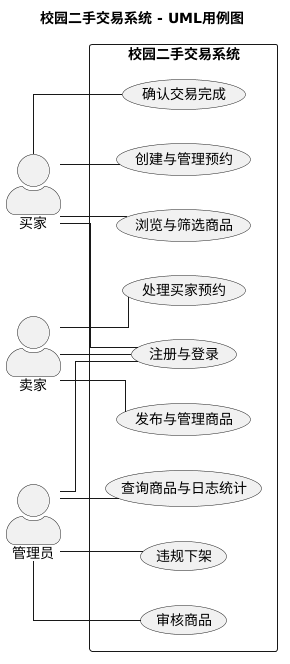
\includegraphics[width=0.3\textwidth]{UML/UML用例图.png}
		\caption{校园二手交易系统 UML 用例图}
		\label{fig:usecase}
	\end{figure}
	
	用例图从用户角色的角度描述系统功能，包含买家、卖家和管理员三类参与者。买家主要负责浏览商品、创建和管理预约以及确认交易完成；卖家主要负责发布和管理商品、处理买家预约；管理员负责商品审核、违规下架以及商品和日志查询。
	
	该图明确了不同角色与系统功能之间的关系，为系统功能模块划分提供依据。
	
	\subsection{类图}
	
	\begin{figure}[H]
		\centering
		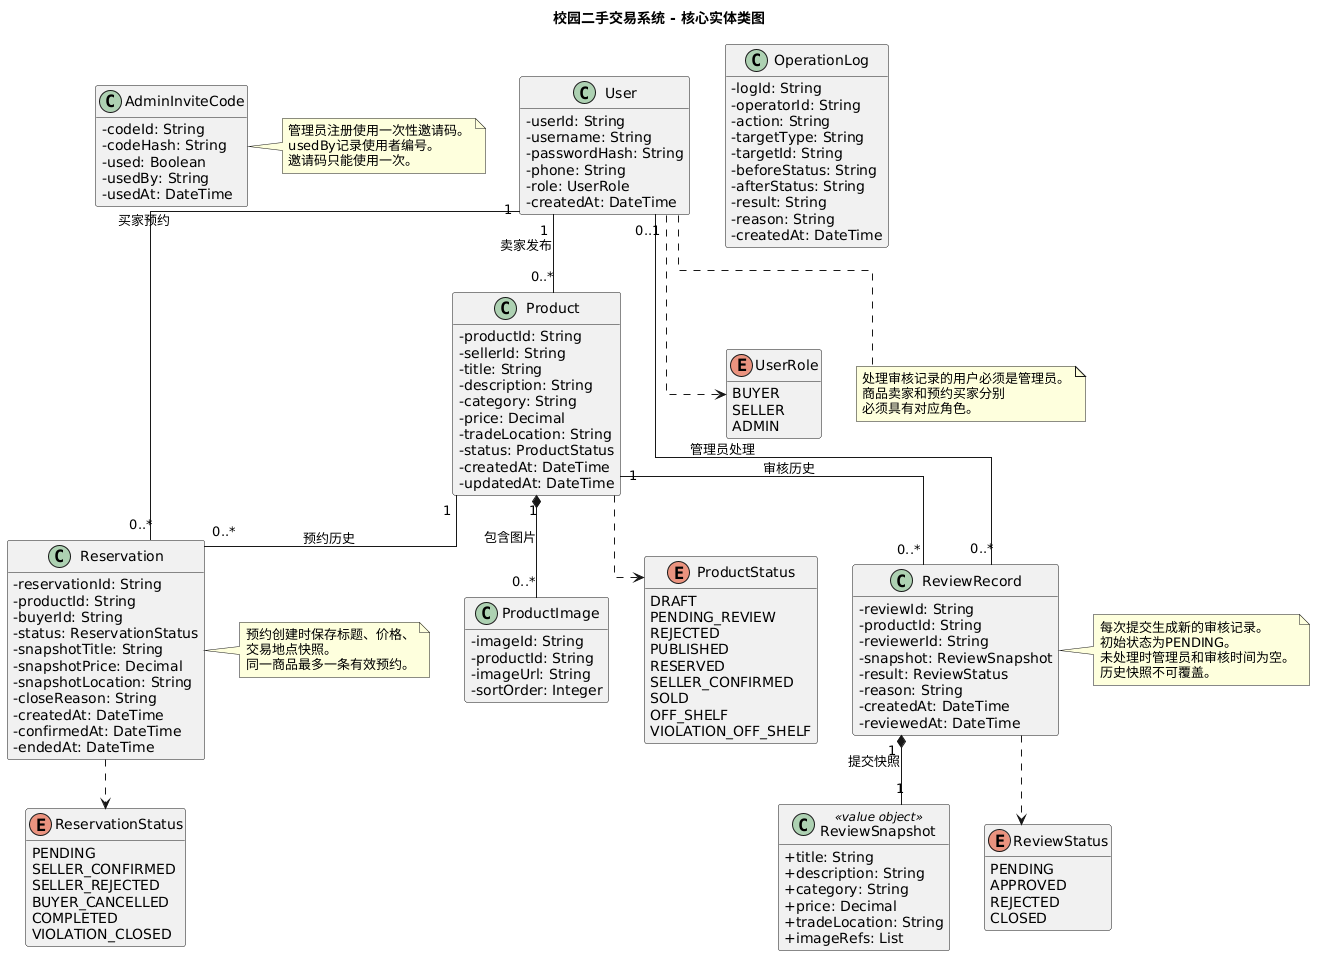
\includegraphics[width=0.92\textwidth]{UML/UML类图.png}
		\caption{校园二手交易系统核心实体类图}
		\label{fig:class}
	\end{figure}
	
	类图主要描述系统中的核心数据实体及其关联关系。
	
	\textbf{（1）User：用户类}
	
	User 类用于描述系统中的用户信息，主要包含用户编号、用户名、密码哈希、联系电话、用户角色和创建时间等属性。用户角色通过 UserRole 枚举表示，包括买家（BUYER）、卖家（SELLER）和管理员（ADMIN）。
	
	设计 User 类的主要原因是将不同角色的公共身份信息统一管理，而不是分别建立买家类、卖家类和管理员类。三种角色均具有账号、密码和联系方式等共同属性，其主要区别在于操作权限，因此使用统一用户实体配合角色枚举，可以减少数据冗余，并便于实现集中式身份认证和权限控制。
	
	\textbf{（2）Product：商品类}
	
	Product 类用于描述卖家发布的二手商品，是系统的核心业务实体之一。其主要属性包括商品编号、卖家编号、商品标题、描述、分类、价格、交易地点、商品状态、创建时间和更新时间。	
	商品状态通过 ProductStatus 枚举表示，包括草稿、待审核、审核驳回、已发布、已预约、卖家已确认、已售出、已下架和违规下架九种状态。
	
	将商品信息集中在 Product 类中，能够统一管理商品从创建、审核、发布到预约交易及最终结束的完整生命周期。	
	商品状态采用枚举类型而不是任意字符串，可以明确状态的取值范围，便于业务逻辑层根据状态判断允许执行的操作，避免非法状态转换。
	
	\textbf{（3）ProductImage：商品图片类}
	
	ProductImage 类用于保存商品图片的相关信息，主要包括图片编号、所属商品编号、图片地址和排序序号。
	Product 与 ProductImage 之间采用一对多的组合关系，即一个商品可以包含多张图片，每张图片只属于一个商品。
	
	将商品图片独立设计为实体类，而不是直接在 Product 中保存多个图片字段，主要是为了支持一个商品对应多张图片的需求，同时避免在商品实体中设置固定数量的图片属性。
	图片排序序号用于确定商品图片的展示顺序，使商品详情界面能够按照预定顺序展示图片。
	
	\textbf{（4）Reservation：预约记录类}
	
	Reservation 类用于描述买家对商品发起的预约，主要属性包括预约编号、商品编号、买家编号、预约状态、商品标题快照、商品价格快照、交易地点快照、关闭原因、创建时间、确认时间和结束时间。
	预约状态通过 ReservationStatus 枚举表示，包括待卖家确认、卖家已确认、卖家已拒绝、买家已取消、已完成和因违规关闭六种状态。
	User 与 Reservation 之间是一对多关系，一个买家可以创建多条预约记录；Product 与 Reservation 之间也是一对多关系，一个商品在不同时间可以产生多条历史预约。
		
	\textbf{（5）ReviewRecord：审核记录类}
	
	ReviewRecord 类用于记录管理员对商品提交信息的审核过程，主要属性包括审核编号、商品编号、审核人编号、审核快照、审核状态、审核原因、创建时间和审核时间。
	审核状态通过 ReviewStatus 枚举表示，包括待审核、审核通过、审核驳回和已关闭四种状态。
	Product 与 ReviewRecord 之间采用一对多关系，一个商品可以对应多条审核记录。
	
	系统规定每次提交审核都创建新的 ReviewRecord，历史记录不被后续审核覆盖，以保证审核过程的可追溯性。
	
	\textbf{（6）ReviewSnapshot：审核快照类}
	
	ReviewSnapshot 是用于保存商品提交审核时信息的值对象，主要包含商品标题、描述、分类、价格、交易地点和图片引用列表等属性。
	ReviewRecord 与 ReviewSnapshot 之间采用一对一的组合关系，每条审核记录包含一份对应的商品信息快照。
	
	将审核快照独立设计为值对象，主要是为了区分商品的当前信息与历史审核时提交的信息。
	通过在每次审核记录中保存独立快照，可以保证管理员能够查看各次审核对应的实际提交内容，同时避免历史审核记录受到后续商品修改的影响。
	
	\textbf{（7）AdminInviteCode：管理员邀请码类}
	
	AdminInviteCode 类用于管理管理员注册时使用的一次性邀请码，主要属性包括邀请码编号、邀请码哈希、是否已使用、使用者编号和使用时间。
	该类与 User 存在关联关系，用于记录邀请码的使用情况及对应的管理员账号。
	
	通过一次性邀请码机制，可以对管理员账号创建过程进行额外限制。
	邀请码使用后记录其使用状态及对应用户，能够防止同一邀请码被重复使用，并为管理员账号创建提供追踪依据。
	
	\textbf{（8）OperationLog：操作日志类}
	
	OperationLog 类用于保存系统关键业务操作的日志信息，主要属性包括日志编号、操作人编号、操作类型、操作对象类型、对象编号、操作前状态、操作后状态、执行结果、操作原因和创建时间。
	
	单独设计 OperationLog 类，是为了将业务操作记录与具体业务实体分离，避免在商品、预约和审核等实体中重复设置日志字段。	
	便于管理员查询历史操作，并为业务问题定位和操作追踪提供依据。
	
	\textbf{（9）枚举类型设计}
	
	除上述实体类外，类图还定义了以下枚举类型：
	
	\begin{itemize}
		\item \textbf{UserRole：}定义 BUYER、SELLER 和 ADMIN 三种用户角色。
		\item \textbf{ProductStatus：}定义商品生命周期中的九种状态。
		\item \textbf{ReservationStatus：}定义预约生命周期中的六种状态。
		\item \textbf{ReviewStatus：}定义审核记录的四种状态。
	\end{itemize}
	
	使用枚举类型能够统一业务状态的表示方式，避免不同模块使用不一致的状态字符串，同时便于进行状态合法性检查和权限判断。
	
	\textbf{（10）类之间的关联关系及设计原因}
	
	核心实体类之间的关联关系主要包括：
	
	\begin{itemize}
		\item \textbf{User 与 Product：}一个卖家可以发布多个商品，每个商品对应一个卖家，体现商品的归属关系。
		\item \textbf{User 与 Reservation：}一个买家可以创建多条预约记录，每条预约对应一个买家，体现预约的发起者。
		\item \textbf{Product 与 ProductImage：}一个商品可以包含多张图片，采用组合关系管理商品图片。
		\item \textbf{Product 与 Reservation：}一个商品可以具有多条历史预约记录，但同一时刻最多存在一条有效预约。
		\item \textbf{Product 与 ReviewRecord：}一个商品可以经历多次审核，每次审核对应独立记录。
		\item \textbf{ReviewRecord 与 ReviewSnapshot：}每条审核记录包含一份提交时的商品信息快照，保证审核历史不受后续修改影响。
		\item \textbf{User 与 ReviewRecord：}审核记录关联执行审核的管理员，用于明确审核责任。
		\item \textbf{AdminInviteCode 与 User：}记录一次性邀请码与管理员账号的使用关联。
	\end{itemize}
	
	\subsection{商品状态图}
	
	\begin{figure}[H]
		\centering
		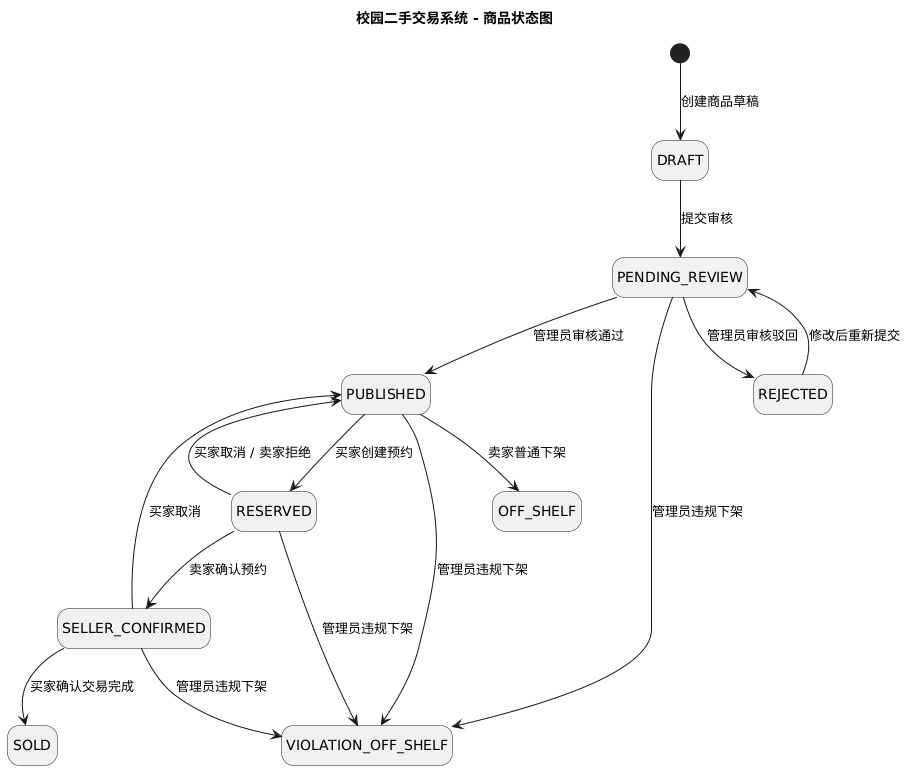
\includegraphics[width=0.82\textwidth]{UML/UML商品状态图.png}
		\caption{校园二手交易系统商品状态图}
		\label{fig:product-state}
	\end{figure}
	
	商品状态图描述商品从创建到最终结束的完整生命周期。
	
	商品首先进入草稿状态，提交审核后进入待审核状态。管理员审核通过后进入已发布状态，审核驳回后进入审核驳回状态，卖家可以修改后重新提交审核。
	
	已发布商品可以被买家预约，预约成功后进入已预约状态；卖家确认预约后进入卖家已确认状态；买家确认交易完成后，商品进入已售出状态。
	
	此外，卖家可以对符合条件的商品执行普通下架，管理员也可以对违规商品执行违规下架。违规下架具有相应的状态约束，并需要同步处理关联预约。
	
	\subsection{预约状态图}
	
	\begin{figure}[H]
		\centering
		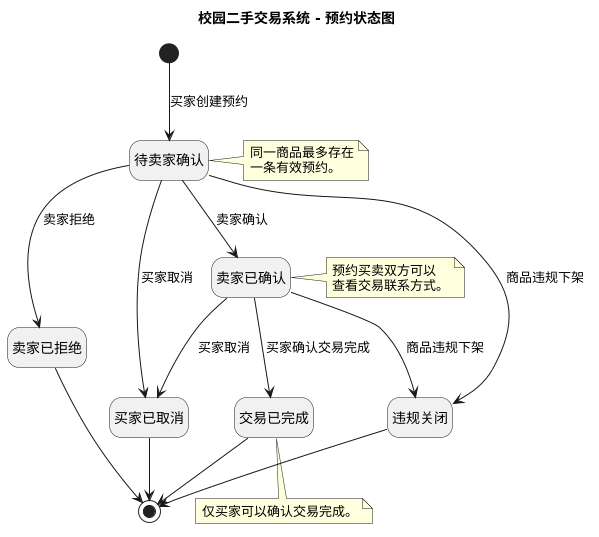
\includegraphics[width=0.82\textwidth]{UML/UML预约状态图.png}
		\caption{校园二手交易系统预约状态图}
		\label{fig:reservation-state}
	\end{figure}
	
	预约状态图描述预约从创建到结束的状态变化过程。
	
	买家创建预约后，预约进入待卖家确认状态。卖家可以确认或拒绝预约；买家可以在允许的状态下取消预约。卖家确认后，买卖双方可以查看交易联系方式，最终由买家确认交易完成。
	
	如果关联商品被管理员违规下架，预约将进入因违规关闭状态。
	
	\subsubsection{预约创建时序图}
	
	\begin{figure}[H]
		\centering
		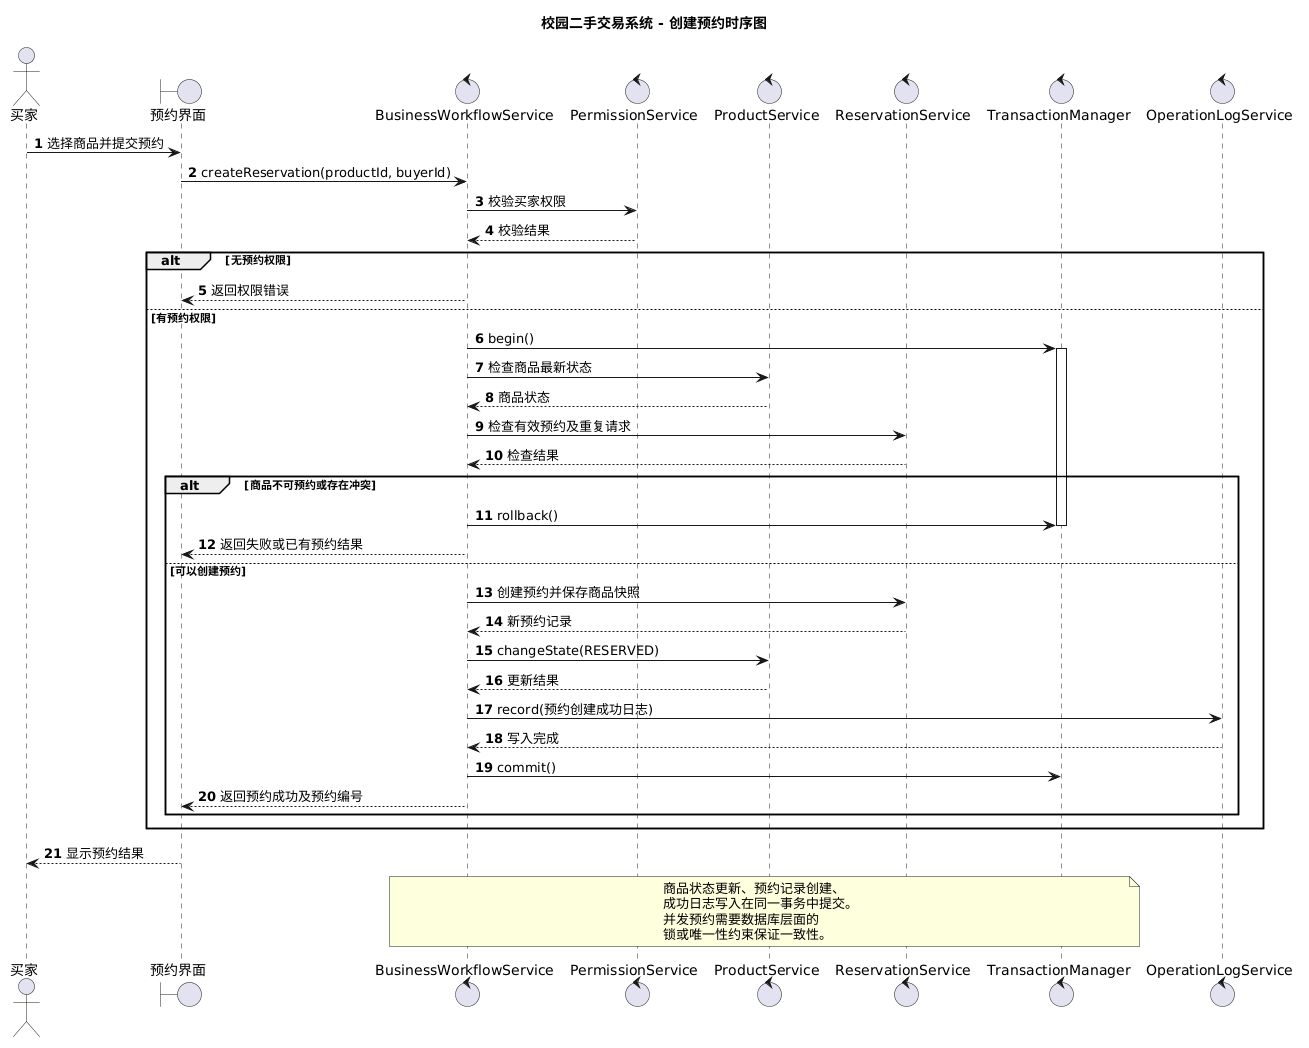
\includegraphics[width=\textwidth]{UML/UML预约创建时序图.png}
		\caption{校园二手交易系统预约创建时序图}
		\label{fig:reservation-sequence}
	\end{figure}
	
	预约创建时序图描述买家发起预约时，各业务组件之间的交互过程。
	
	买家通过预约界面提交商品编号和用户编号后，BusinessWorkflowService 首先调用 PermissionService 验证买家权限。权限验证通过后，启动事务，并分别调用 ProductService 检查商品当前状态、调用 ReservationService 检查是否存在有效预约及重复请求。
	
	检查通过后，ReservationService 创建预约记录并保存商品信息快照，ProductService 将商品状态更新为 RESERVED，OperationLogService 记录预约创建成功日志。最后由 TransactionManager 提交事务，并将预约结果返回给预约界面。
	
	如果权限验证失败，系统返回权限错误；如果商品不可预约或预约存在冲突，则执行事务回滚，不产生部分成功的业务数据。
	
	\section{UI界面及功能描述}
	
	\begin{table}[H]
		\centering
		\caption{UI界面与系统功能模块对应关系}
		\label{tab:ui-module}
		\renewcommand{\arraystretch}{1.35}
		\begin{tabular}{
				>{\raggedright\arraybackslash}p{0.25\textwidth}
				>{\raggedright\arraybackslash}p{0.58\textwidth}
			}
			\toprule
			\textbf{UI界面} & \textbf{对应功能模块} \\
			\midrule
			登录注册界面 & 用户与权限管理 \\
			商品首页界面 & 商品查询 \\
			商品列表与搜索界面 & 商品查询 \\
			商品详情界面 & 商品查询、预约与交易管理 \\
			发布闲置界面 & 商品管理 \\
			个人中心界面 & 用户与权限管理、商品管理、预约与交易管理 \\
			我的商品界面 & 商品管理 \\
			我的预约界面 & 预约与交易管理 \\
			管理员审核界面 & 商品审核 \\
			\bottomrule
		\end{tabular}
	\end{table}
	
	\subsection{登录注册界面}
	
	登录注册界面如图~\ref{fig:ui-login}所示。
	
	\begin{figure}[H]
		\centering
		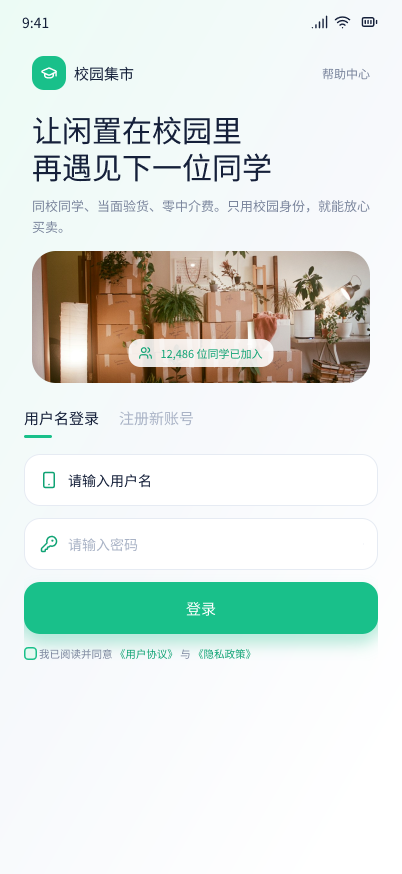
\includegraphics[
		width=0.48\textwidth,
		height=0.72\textheight,
		keepaspectratio
		]{UI界面/UI界面1.png}
		\caption{登录注册界面}
		\label{fig:ui-login}
	\end{figure}
	
	该界面对应用户与权限管理模块，
	用于提供系统用户的身份认证入口。
	
	界面顶部展示系统名称和宣传信息，
	中部设置用户名与密码输入框，
	并提供登录按钮及注册新账号入口。
	用户输入账号信息后，可以通过登录按钮
	提交身份验证请求。
	
	在注册流程中，系统根据用户选择的角色
	完成相应的账号创建与权限配置。
	对于管理员角色，系统还需要按照业务规则
	验证一次性管理员邀请码。
	
	\subsection{商品首页界面}
	
	商品首页界面如图~\ref{fig:ui-home}所示。
	
	\begin{figure}[H]
		\centering
		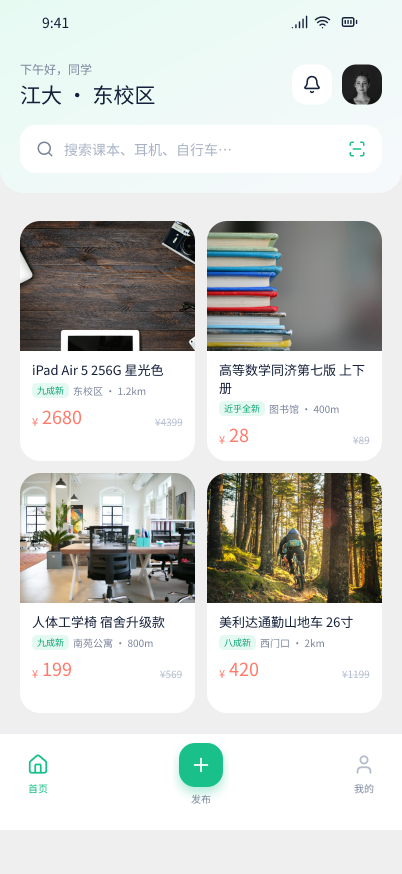
\includegraphics[
		width=0.48\textwidth,
		height=0.72\textheight,
		keepaspectratio
		]{UI界面/UI界面2.png}
		\caption{商品首页界面}
		\label{fig:ui-home}
	\end{figure}
	
	该界面对应商品查询模块。
	
	界面顶部展示用户问候信息、所在校区、
	搜索框和个人头像等内容。
	用户可以通过搜索框输入商品关键词，
	进入相应的商品查询结果页面。
	
	页面主体采用双列商品卡片布局，
	展示商品图片、标题、新旧程度、
	交易区域和出售价格等信息。
	每张商品卡片均可作为商品详情的入口，
	方便用户进一步查看商品信息。
	
	底部设置首页、发布和个人中心等导航入口，
	便于用户在商品浏览、商品发布和个人业务管理
	之间进行切换。
	
	首页重点展示商品的图片、名称和价格，
	使用户能够快速了解商品的基本情况，
	减少查找目标商品所需的操作步骤。
	
	\subsection{商品列表与搜索界面}
	
	商品列表与搜索界面如图~\ref{fig:ui-list}所示。
	
	\begin{figure}[H]
		\centering
		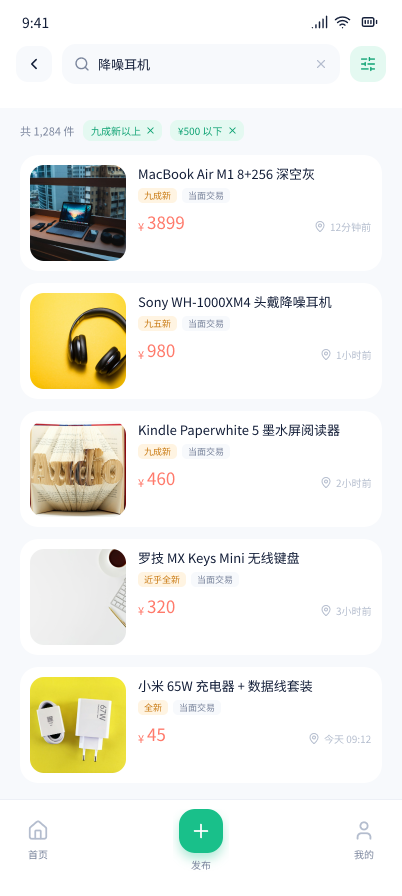
\includegraphics[
		width=0.48\textwidth,
		height=0.72\textheight,
		keepaspectratio
		]{UI界面/UI界面3.png}
		\caption{商品列表与搜索界面}
		\label{fig:ui-list}
	\end{figure}
	
	该界面对应商品查询模块，
	用于展示符合搜索条件的商品信息。
	
	界面顶部设置搜索输入框和筛选入口，
	用户可以输入商品关键词，
	并根据商品价格范围等条件
	筛选。
	
	搜索条件以标签形式显示在商品列表上方，
	便于用户查看当前筛选条件，
	并通过标签上的删除入口取消对应条件。
	
	商品列表采用纵向卡片布局，
	每条商品记录展示商品图片、名称、
	价格及发布时间等信息。
	
	用户选择某一商品后，
	可以进入商品详情界面查看完整信息。
	
	\subsection{商品详情界面}
	
	商品详情界面如图~\ref{fig:ui-detail}所示。
	
	\begin{figure}[H]
		\centering
		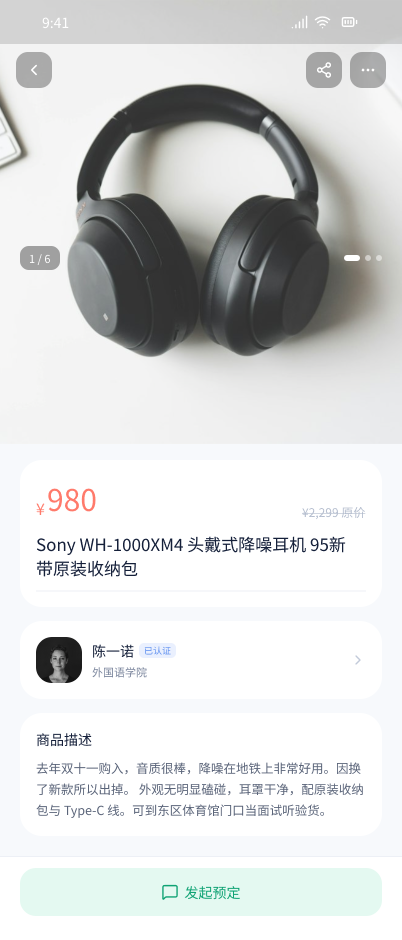
\includegraphics[
		width=0.48\textwidth,
		height=0.72\textheight,
		keepaspectratio
		]{UI界面/UI界面4.png}
		\caption{商品详情界面}
		\label{fig:ui-detail}
	\end{figure}
	
	商品详情界面对应商品查询模块和
	预约与交易管理模块，
	用于展示商品完整信息并提供预约入口。
	
	界面顶部设置商品图片展示区域，
	通过图片序号和切换指示展示多张商品图片。
	
	商品信息区域展示商品价格、标题、
	新旧程度和其他基本信息。
	卖家信息区域展示卖家头像、用户名及所属信息，
	便于买家了解商品发布者。
	
	商品描述区域用于展示卖家填写的商品详细说明，
	帮助买家判断商品是否符合购买需求。
	
	界面底部设置“发起预定”按钮。
	当商品处于允许预约的状态时，
	买家可以通过该入口提交预约请求。
	
	预约请求由业务逻辑层进行权限验证、
	商品状态检查和有效预约冲突检查。
	预约成功后，系统创建预约记录，
	并将商品状态更新为已预约。
	
	该界面将商品展示与预约操作结合，
	使买家能够在了解商品信息后直接发起预约，
	减少页面切换。
	
	\subsection{发布闲置界面}
	
	发布闲置界面如图~\ref{fig:ui-publish}所示。
	
	\begin{figure}[H]
		\centering
		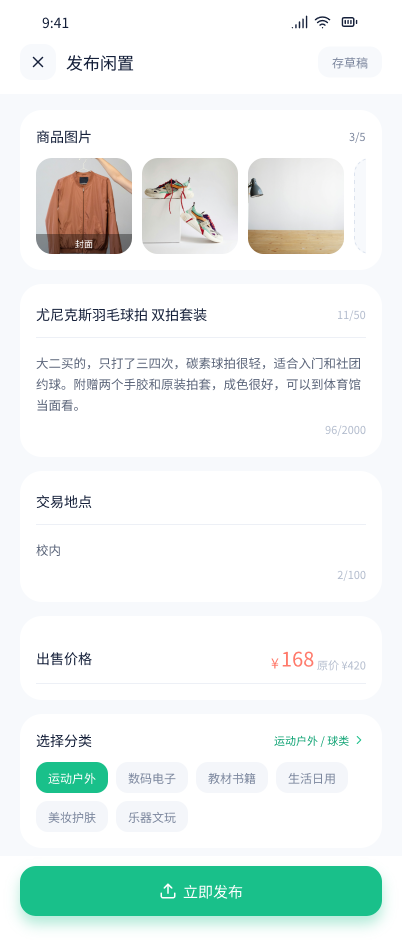
\includegraphics[
		width=0.48\textwidth,
		height=0.72\textheight,
		keepaspectratio
		]{UI界面/UI界面5.png}
		\caption{发布闲置界面}
		\label{fig:ui-publish}
	\end{figure}
	
	发布闲置界面对应商品管理模块，
	主要面向卖家，用于创建和提交商品信息。
	将商品信息划分为多个独立填写区域，
	主要包括以下内容：
	
	\begin{itemize}
		\item \textbf{商品图片：}
		上传并展示商品图片，
		通过图片数量提示显示当前上传情况。
		
		\item \textbf{商品标题与描述：}
		填写商品名称和详细说明，
		并通过字数提示控制输入长度。
		
		\item \textbf{交易地点：}
		填写线下交易地点，
		便于买卖双方确定交接位置。
		
		\item \textbf{出售价格：}
		设置商品出售价格，
		界面同时提供原价信息展示区域。
		
		\item \textbf{商品分类：}
		通过分类标签选择商品所属类别，
		便于后续商品筛选和查询。
	\end{itemize}
	
	界面顶部提供“存草稿”入口，
	用于保存尚未完成的商品信息；
	底部设置“立即发布”按钮，
	用于提交完整的商品信息。
	
	商品提交后进入待审核状态。
	管理员审核通过后，
	商品才进入已发布状态。
	
	该界面将图片、文字描述、价格、
	交易地点和分类分别组织，
	有助于减少信息填写遗漏，
	同时与商品实体类中的主要属性保持一致。
	
	\subsection{个人中心界面}
	
	个人中心界面如图~\ref{fig:ui-profile}所示。
	
	\begin{figure}[H]
		\centering
		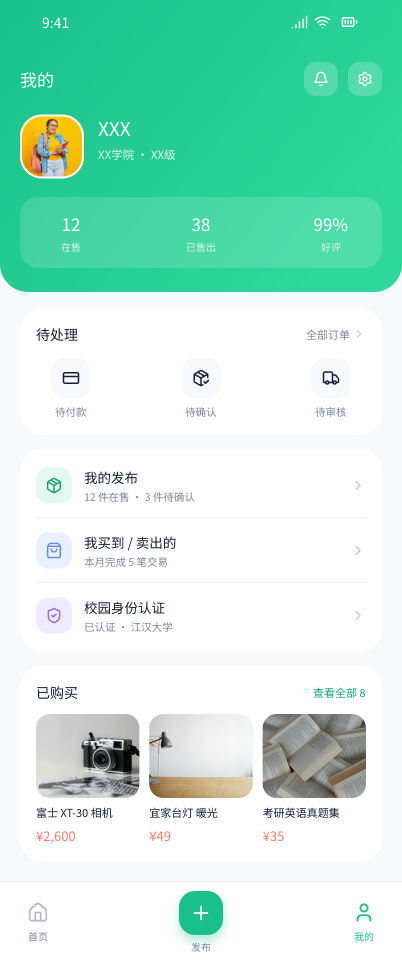
\includegraphics[
		width=0.48\textwidth,
		height=0.72\textheight,
		keepaspectratio
		]{UI界面/UI界面6.png}
		\caption{个人中心界面}
		\label{fig:ui-profile}
	\end{figure}
	
	个人中心界面用于集中展示当前用户的
	个人信息和相关业务入口，
	涉及用户与权限管理、商品管理以及
	预约与交易管理等多个模块。
	
	界面顶部展示用户头像、用户名及个人业务统计信息。
	
	中部设置待处理事项区域，
	以图标和文字形式展示需要用户关注的业务。
	
	功能列表提供“我的发布”
	和“我买到／卖出的”等入口，
	分别对应商品管理和交易记录查询功能。
	
	界面下方展示部分历史商品记录，
	便于用户快速查看相关商品信息。
	
	通过将个人信息、待处理事项和业务入口
	集中在同一页面，
	用户可以快速进入相应功能模块，
	避免在多个页面之间反复查找。
	
	\subsection{我的商品界面}
	
	我的商品界面如图~\ref{fig:ui-products}所示。
	
	\begin{figure}[H]
		\centering
		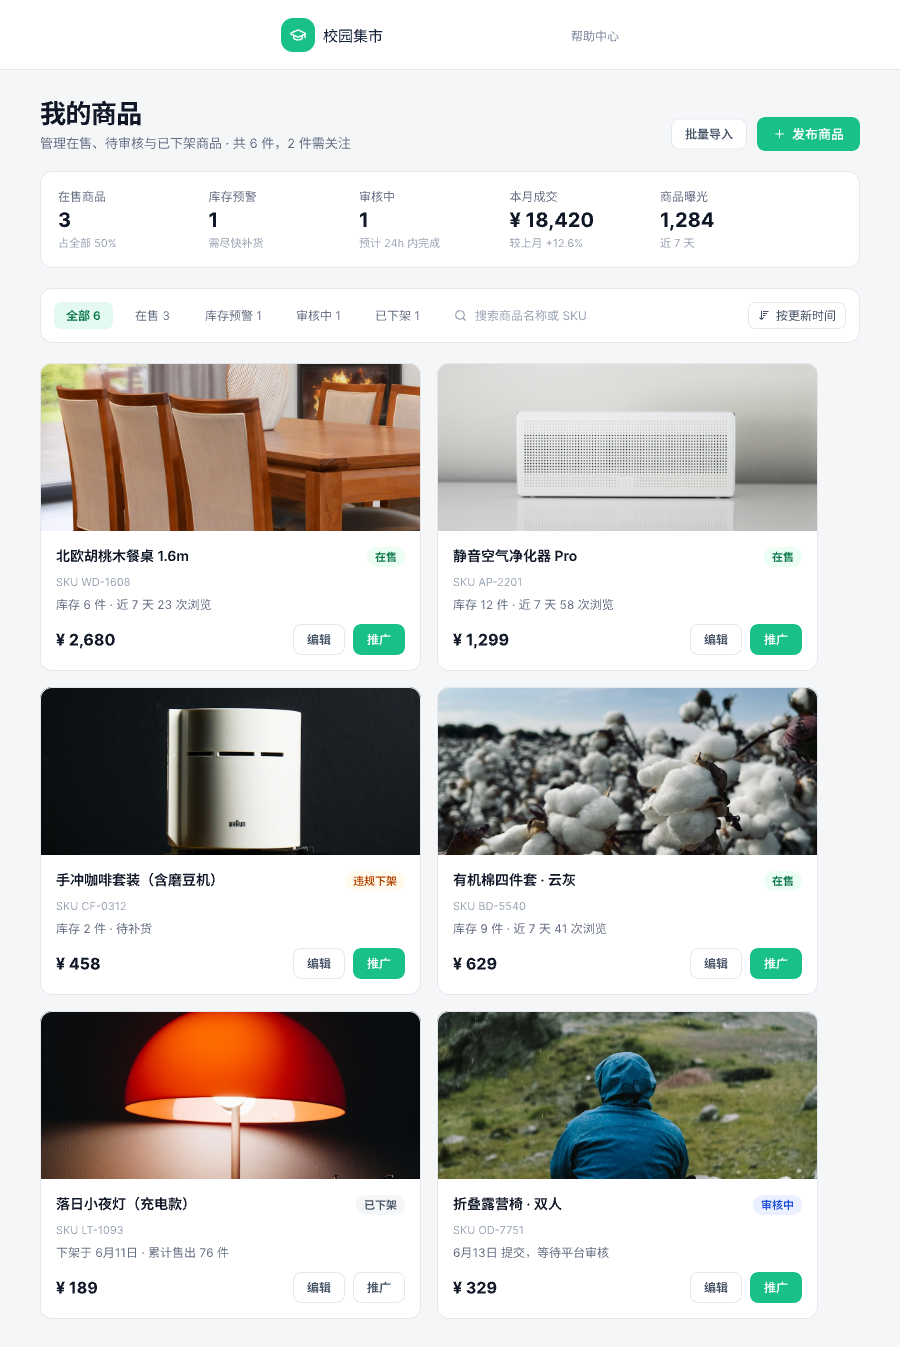
\includegraphics[
		width=0.95\textwidth,
		height=0.78\textheight,
		keepaspectratio
		]{UI界面/UI界面7.png}
		\caption{我的商品管理界面}
		\label{fig:ui-products}
	\end{figure}
	
	我的商品界面对应商品管理模块，
	用于卖家集中查看和管理自己发布的商品。
	
	界面顶部展示商品管理标题、
	商品数量及相关统计信息，
	并提供发布商品入口。
	
	商品列表上方设置状态筛选区域，
	用户可以按照在售、审核中、
	已下架等状态查看商品。
	
	该界面将商品状态和管理操作集中展示，
	便于卖家了解商品当前所处的业务阶段，
	并对多个商品进行统一管理。
	
	\subsection{我的预约界面}
	
	我的预约界面如图~\ref{fig:ui-reservations}所示。
	
	\begin{figure}[H]
		\centering
		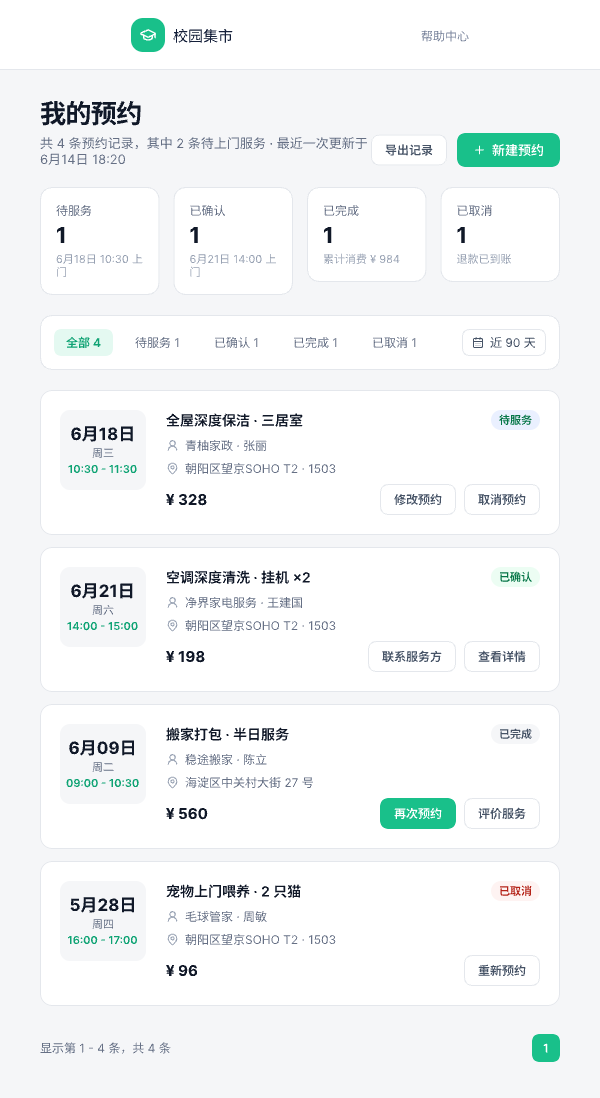
\includegraphics[
		width=0.95\textwidth,
		height=0.78\textheight,
		keepaspectratio
		]{UI界面/UI界面8.png}
		\caption{我的预约管理界面}
		\label{fig:ui-reservations}
	\end{figure}
	
	我的预约界面对应预约与交易管理模块，
	用于展示用户的预约记录及其处理状态。
	
	界面顶部设置预约统计卡片，
	用于展示不同状态下的预约数量，
	便于用户了解当前预约情况。
	
	在系统业务设计中，
	预约状态包括待卖家确认、卖家已确认、
	卖家已拒绝、买家已取消、
	已完成和因违规关闭六种状态。
	不同状态对应不同的业务操作，预约管理界面需要根据
	当前用户角色和预约状态，
	动态展示允许执行的操作。
	
	该界面通过状态标签、分类筛选
	和操作按钮组织预约记录，
	使用户能够直观了解预约进度。
	
	\subsection{管理员审核界面}
	
	管理员审核界面如图~\ref{fig:ui-admin}所示。
	
	\begin{figure}[H]
		\centering
		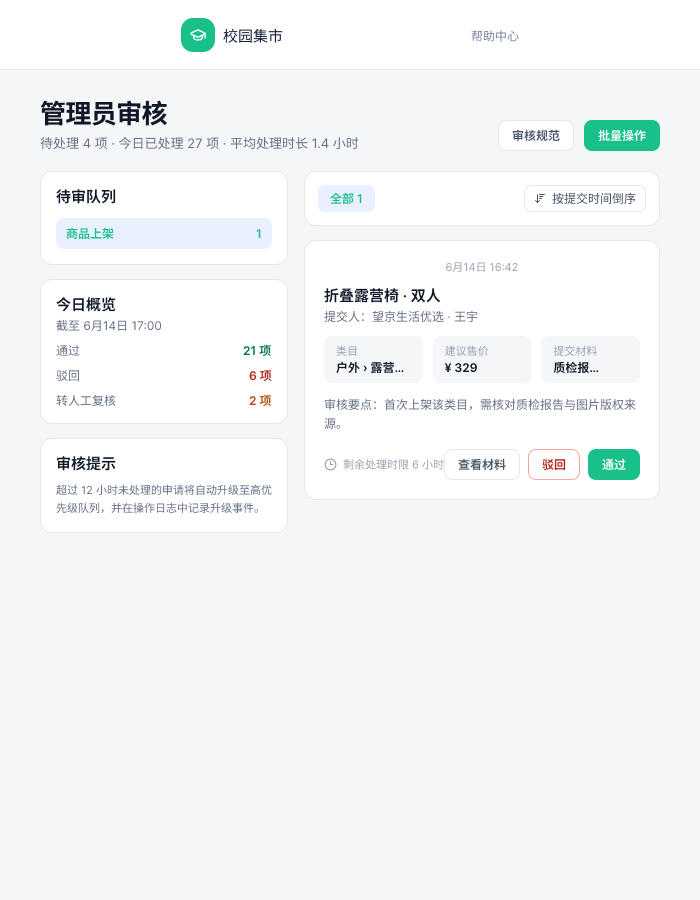
\includegraphics[
		width=0.95\textwidth,
		height=0.78\textheight,
		keepaspectratio
		]{UI界面/UI界面9.png}
		\caption{管理员商品审核界面}
		\label{fig:ui-admin}
	\end{figure}
	
	管理员审核界面对应商品审核模块，
	主要用于管理员查看和处理待审核商品。
	
	界面采用桌面端布局，
	将审核任务列表、审核统计信息
	和具体审核内容分区展示。
	
	左侧设置待审队列、今日概览
	和审核提示等区域，
	用于展示当前审核任务数量
	以及审核工作的整体情况。
	
	右侧为商品审核区域，
	展示商品名称、提交人、
	商品分类、建议售价及提交材料等信息。
	
	审核通过后，
	商品状态由待审核变为已发布；
	审核驳回后，
	商品状态变为审核驳回，
	同时保存相应的审核原因。
	
	系统为每次审核提交创建独立的审核记录，
	并保存商品提交时的信息快照，
	以保证审核历史的完整性。
	
	\subsection{管理员操作日志界面}
	
	管理员操作日志界面如图~\ref{fig:ui-log}所示。
	
	\begin{figure}[H]
		\centering
		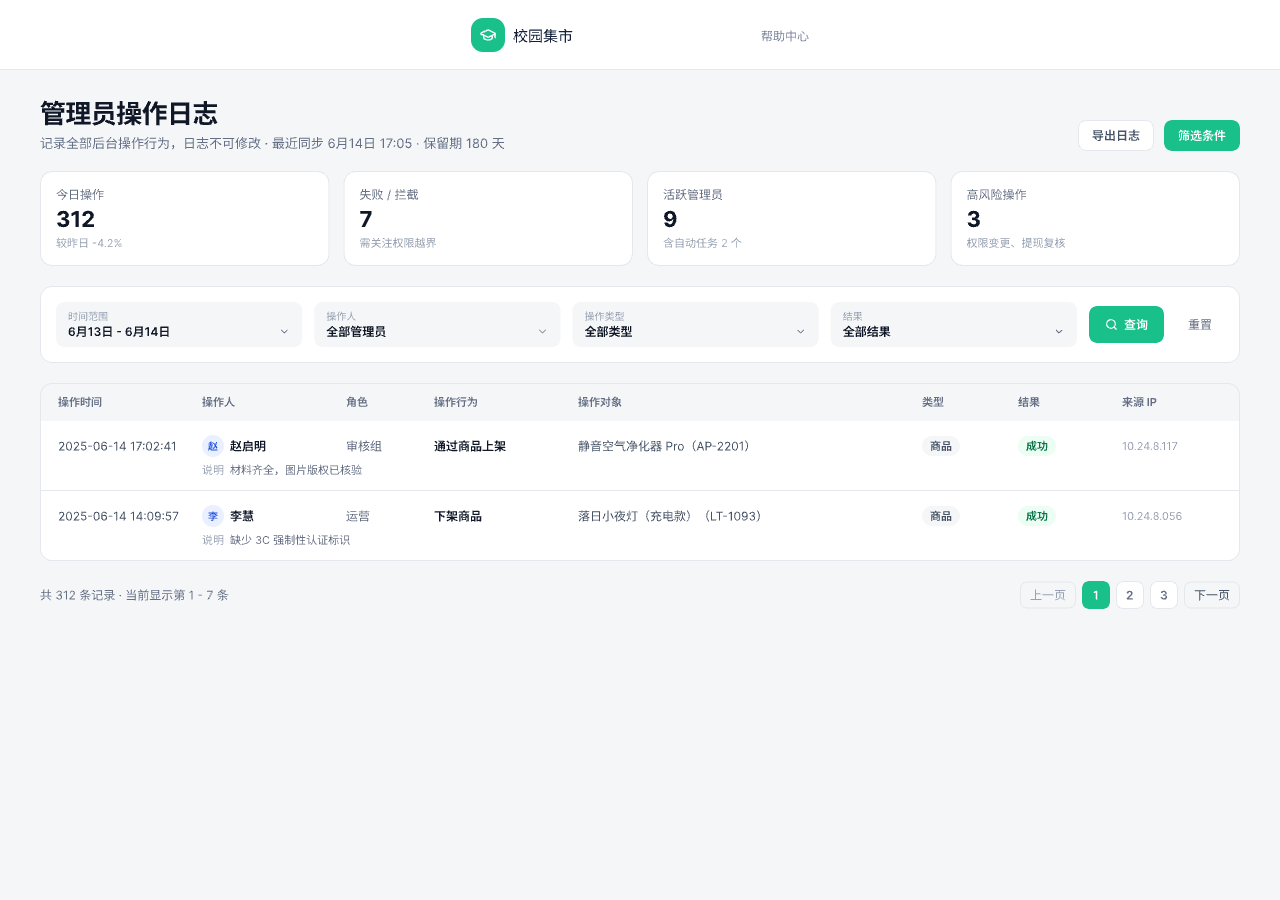
\includegraphics[
		width=0.95\textwidth,
		height=0.78\textheight,
		keepaspectratio
		]{UI界面/UI界面10.png}
		\caption{管理员操作日志界面}
		\label{fig:ui-log}
	\end{figure}
	
	管理员操作日志界面对应统计与日志管理模块，
	主要用于管理员查询和追踪系统中的关键业务操作，
	为系统运行管理、问题定位和操作审计提供支持。
	
	根据系统核心实体类图中的 OperationLog 类，
	每条日志主要记录操作人编号、操作类型、
	操作对象类型、对象编号、操作前状态、
	操作后状态、执行结果、操作原因和创建时间等信息。
	
	该界面通过统计卡片、组合筛选和表格展示，
	使管理员既能了解整体操作情况，
	又能定位具体业务操作记录，
	提高系统操作的可追溯性和管理便利性。
	
	\section{辅助工具的使用与分析}
	
	\subsection{功能分析}
	
	在本次实验中，我使用 ChatGPT 辅助分析实验一完成的需求分析报告，梳理校园二手交易系统的主要功能，并结合实验要求，将系统划分为用户与权限管理、商品管理、商品查询、预约与交易管理、商品审核与违规处理、统计与日志管理六个核心模块。
	
	这一过程帮助我进一步理解了需求分析与软件设计之间的关系，使系统功能划分更加清晰，也为后续 UML 建模提供了依据。
	
	\subsection{软件架构 UML 图}
	
	在 UML 设计过程中，我主要使用 ChatGPT 辅助梳理系统结构、分析实体关系和生成 PlantUML 代码，并通过 PlantUML 工具绘制和调整 UML 图。
	
	本次实验共设计了六张 UML 图，包括用例图、组件图、核心实体类图、商品状态图、预约状态图和预约创建时序图。
	
	在设计过程中，我对大模型生成的初始方案进行了多次修改和优化。例如，在类图设计中，最初的方案包含较多业务服务类，导致类图内容复杂、关联关系不够直观。经过分析，我将类图重点调整为核心实体及其关系，保留用户、商品、预约、审核记录、操作日志等实体，并通过独立的状态枚举和快照对象描述业务规则。
	
	在状态图设计中，我重点检查了商品和预约的状态转换是否符合需求，明确了预约取消、卖家确认、交易完成和违规下架等操作对应的状态变化。在时序图设计中，我进一步考虑了预约创建过程中的权限验证、商品状态检查、预约冲突检查和事务管理，避免只描述正常流程而忽略异常情况。
	
	\subsection{UI 界面设计}
	
	在 UI 设计方面，我主要使用 Pixso 及其内置 AI 工具生成界面原型。	
	根据系统的主要功能，我设计了登录注册、商品首页、商品列表、商品详情、发布闲置、个人中心、我的商品、我的预约、管理员审核和管理员操作日志十个界面。
	
	在设计过程中，我首先根据需求分析和 UML 图明确各界面需要展示的信息和操作入口，再将这些要求整理为提示词输入 Pixso AI，生成初步界面。随后，我对生成结果进行了检查和修改。
	
	例如，最初生成的登录界面采用手机号验证码登录，与需求中设计的用户名和密码登录方式不一致，因此将其调整为用户名和密码输入。商品发布界面也根据 Product 类中的属性，调整了商品标题、描述、图片、价格、分类和交易地点等输入内容。
	
	\subsection{辅助工具的优缺点分析}
	
	（1）优点
	
	提高设计效率:
	
	大模型能够快速整理需求、生成 PlantUML 代码和 UI 设计提示词，减少重复性工作，使我能够将更多时间投入到业务规则分析和设计优化中。
	
	辅助理解软件设计方法:
	
	通过与大模型讨论 UML 图的组成、实体关系和模块职责，我对软件架构设计和 UML 建模方法有了更深入的理解。
	
	降低 UI 设计门槛:
	
	Pixso AI 能够根据文字描述快速生成较为完整的界面原型，帮助我建立统一的视觉风格，并快速尝试不同的布局方案。
	
	（2）缺点
	
	生成结果偏离实际需求：
	
	Pixso AI 根据常见电商系统的特点自动补充在线支付、库存管理、推广等功能，但这些功能并不属于本系统的需求范围。
	
	工具之间的结果不一致：
	
	UML 图强调业务规则和数据关系，而 UI 生成工具更侧重视觉效果，导致界面中的功能与系统设计不一致，需要人工统一。
	
	（3）总结
	
	总体而言，本次实验中辅助工具主要发挥了需求梳理、绘图辅助和界面设计的作用。通过使用 ChatGPT 和 Pixso AI，我提高了软件设计的效率，同时也发现 AI 生成结果并不一定符合具体业务需求。
	
	因此，在实际使用过程中，需要根据实验一的需求分析报告和本次实验的设计要求，对生成内容进行检查、筛选和修改。
	
\end{document}